\subsection{Breitensuche}

In diesem Abschnitt diskutieren wir eine alternative Methode zur Graphendurchmusterung.
Im Gegensatz zur Tiefensuche besteht der Ansatz darin, zuerst die ganze direkte Nachbarschaft eines Knotens abzusuchen, bevor man tiefer in den Graphen hineinsieht.
Daher wird die Methode als \emph{Breitensuche} bezeichnet, und nach dem englischen Begriff \emph{depth first search} oft einfach \emph{BFS} genannt.

Wie wir sehen werden erlaubt uns diese Strategie andere Eigenschaften des betrachteten (Di)Graphen zu erkunden.
Die wichtigste unter ihnen ist sicherlich das Bestimmen der Länge und das Auffinden von kürzesten Pfaden, die ausgehend von einem festgelegten Startknoten einen anderen Knoten im (Di)Graphen verbinden.

Die Eingabe für die Breitensuche ist ein Digraph $D=(V,A)$, der wie bei der Tiefensuche in Form einer Adjazenzliste gegeben ist.
Auf ungerichteten Graphen ist die Vorgehensweise wiederum analog und wir diskutieren (fast ausschließlich) die gerichtete Variante.

Für zwei Knoten $u,v \in V$ in~$D$ definieren wir den \emph{Abstand} von~$u$ nach~$v$ als die minimale Länge eines $(u,v)$-Pfades und bezeichnen ihn mit $\delta(u,v)$.
Wenn kein solcher Pfad existiert, setzen wir $\delta(u,v):=\infty$.
Für ungerichtete Graphen ist $\delta(u,v)$ entsprechend definiert und es gilt $\delta(u,v)=\delta(v,u)$ für alle Knoten $u,v \in V$.
Wie oben erwähnt erlaubt uns die Breitensuche das Bestimmen der Abstände $\delta(s,v)$ von einem festen \emph{Startknoten} $s \in V$ aus zu jedem anderen Knoten~$v$.
Ist $\delta(s,v) < \infty$, so sagen wir, dass~$v$ von~$s$ aus \emph{erreichbar} ist.

Während der Durchmusterung des Digraphen~$D$ wird ein Array~$d$ der Länge~$|V|$ verwaltet, in dem nach Abschluss der Breitensuche die Abstände $\delta(s,v)$, für alle Knoten $v \in V$, gespeichert sind.

Für die Umsetzung der Breitensuche wird die folgende Hilfsdatenstruktur benutzt.
Eine \emph{Warteschlange}~$Q$ ist eine Liste $Q=[q_1,\ldots,q_k]$, die mit zwei Grundoperationen ausgestattet ist:
\begin{itemize}
 \item $\cc{Dequeue}(Q)$: Das \emph{erste} Element~$q_1$ von~$Q$ wird zurückgegeben und aus der Warteschlange entfernt.
 Man nennt das Element~$q_1$ den \emph{Kopf} der Warteschlange und nach der Operation gilt $Q=[q_2,\ldots,q_k]$.

 \item $\cc{Enqueue}(Q,x)$: Das Element~$x$ wird am \emph{Ende} von~$Q$ hinzugefügt.
 Nach der Ausführung dieser Operation gilt also $Q=[q_1,\ldots,q_k,x]$. 
\end{itemize}

Aufgrund der Einfüge- und Rückgabereihenfolge sagt man auch, dass Warteschlangen nach dem FIFO-Prinzip (First In - First Out) arbeiten.
Warteschlangen mit höchstens $n \in \N$ Elementen können auf der Basis von Arrays der Länge~$n$ umgesetzt werden, sodass die Laufzeit der beiden Grundoperationen $\Theta(1)$ Zeiteinheiten beträgt. 

Bevor wir mit der eigentlichen Breitensuche beginnen können, müssen eine Reihe von Attributen und natürlich auch die Warteschlange korrekt initialisiert werden:
Zu Beginn setzen wir $d[v]:=\infty$, für alle $v \in V \setminus \{s\}$, und $d[s]:=0$.
Besteht die Gleichheit $d[v]=\infty$ zu einem Moment der Breitensuche, so bedeutet dies, dass der Knoten~$v$ bisher noch nicht entdeckt wurde.
Die erste Veränderung des Wertes~$d[v]$ entspricht der Entdeckung von~$v$, und wir nennen $d[v]$ die \emph{aktuelle Distanz} von~$s$ zu~$v$. 
Wir verwalten weiterhin wie bei der Tiefensuche das Farbattribut $\cc{Farbe}[u]$ eines Knotens~$u \in V$ um den Bearbeitungszustand von~$u$ zu jedem Zeitpunkt der Breitensuche zu kennen.
Auch die Vorgängerabbildung~$\pi$ kommt wieder zum Einsatz.

Wir fassen die Initialisierungen zu einer eigenen Hilfsprozedur zusammen:

\begin{algorithm}[H]
\caption{$\cc{Breitensuche-initialisieren}(D,s)$}
\begin{algorithmic}[1]
 \FOR{$u \in V \setminus \{s\}$}
  \STATE $\cc{Farbe}[u] := \cc{weiss}$
  \STATE $d[u] := \infty$ $\quad$ \COMMENT{Aktueller Abstand zu $s$}
  \STATE $\pi[u] := \cc{nil}$ $\quad$ \COMMENT{Vorgänger von $u$}
 \ENDFOR
 \STATE $\cc{Farbe}[s] := \cc{grau}$
 \STATE $d[s] := 0$
 \STATE $\pi[s] := \cc{nil}$
 \STATE Deklariere eine leere Warteschlange $Q$
 \STATE $\cc{Enqueue}(Q,s)$
\end{algorithmic}
\end{algorithm}

Sobald diese Vorbereitung abgeschlossen ist, verläuft die Breitensuche nun wie folgt:
Ausgehend vom Startknoten~$s$ werden zunächst alle Knoten in Abstand~$1$ untersucht, in die Warteschlange eingefügt, und grau gefärbt.
Anschließend wird der erste Nachbarknoten von~$s$ als Ausgangspunkt für die weitere Durchmusterung benutzt, bei der zuerst all seine direkten und noch nicht bereits entdeckten Nachbarn in die Warteschlange eingefügt werden.
Bevor diese Nachbarn genauer untersucht werden, arbeitet der Algorithmus aber erst alle anderen Nachbarn von~$s$ entsprechend ab.
Iterativ werden somit erst alle Knoten mit Distanz~$k$ zu~$s$ besucht, bevor irgendein Knoten in Distanz~$k+1$ untersucht wird.
Das Farbattribut dient zur Unterscheidung der Zustände der Knoten, insbesondere stellen alle aktuell grauen Knoten die jeweilige Front zwischen den entdeckten und den noch unentdeckten Knoten dar.

\begin{algorithm}[H]
\caption{$\cc{Breitensuche}(s)$}
\begin{algorithmic}[1]
 \STATE $\cc{Breitensuche-initialisieren}(s)$
 \WHILE{$Q$ enthält Knoten}
  \STATE\label{line:breitensuche-dequeue} $u:=\cc{Dequeue}(Q)$ $\quad$ \COMMENT{Die Bearbeitung des Knotens $u$ beginnt.}
  \STATE \COMMENT{Aus $u$ ausgehende Kanten werden sondiert}
  \FOR{$v \in N[u]$}
   \IF{$\cc{Farbe}[v]=\cc{weiss}$}\label{line:breitensuche-if}
    \STATE $\cc{Farbe}[v]:=\cc{grau}$
    \STATE\label{line:breitensuche-enqueue} $\cc{Enqueue}(Q,v)$
    \STATE\label{line:breitensuche-pi} $\pi[v] := u$
    \STATE\label{line:breitensuche-d} $d[v]:=d[u]+1$
   \ENDIF
  \ENDFOR
  \STATE $\cc{Farbe}[u]:=\cc{schwarz}$
 \ENDWHILE
\end{algorithmic}
\end{algorithm}

Beachten Sie, dass wir, im Gegensatz zur in Abschnitt~\ref{sect:tiefensuche} diskutierten Tiefensuche, die Breitensuche hier nur \glqq lokal\grqq\ von einem Startknoten~$s$ aus betrachten, und nicht vollständig auf dem gesamten Digraphen betreiben.
Gibt es mehrere (starke) Zusammenhangskomponenten im Digraphen, dann kann die Breitensuche natürlich ausgehend von einem Knoten einer jeden weiteren Komponente neu gestartet werden.

\begin{beispiel}
\label{bsp:breitensuche}
Zum Vergleich mit der Tiefensuche sehen wir uns die Arbeitsweise der Breitensuche wieder auf dem Digaphen aus Beispiel~\ref{bsp:tiefensuche} an:

\hfill
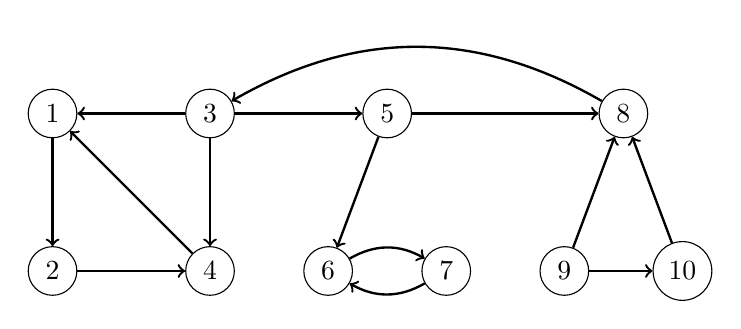
\begin{tikzpicture}[]
 \node[circle,draw=black] (1) at (0,2) {$1$};
 \node[circle,draw=black] (2) at (0,0) {$2$};
 \node[circle,draw=black] (3) at (2,2) {$3$};
 \node[circle,draw=black] (4) at (2,0) {$4$};
 \node[circle,draw=black] (5) at (4.25,2) {$5$};
 \node[circle,draw=black] (6) at (3.5,0) {$6$};
 \node[circle,draw=black] (7) at (5,0) {$7$};
 \node[circle,draw=black] (8) at (7.25,2) {$8$};
 \node[circle,draw=black] (9) at (6.5,0) {$9$};
 \node[circle,draw=black] (10) at (8,0) {$10$};
		
 \draw[->,line width=0.3mm] (1) edge (2);
 \draw[->,line width=0.3mm] (2) edge (4);
 \draw[->,line width=0.3mm] (3) edge (1) (3) edge (4) (3) edge (5);
 \draw[->,line width=0.3mm] (4) edge (1);
 \draw[->,line width=0.3mm] (5) edge (6) (5) edge (8); 
 \draw[->,line width=0.3mm] (6) to[bend left] (7);
 \draw[->,line width=0.3mm] (7) to[bend left] (6);
 \draw[->,line width=0.3mm] (8) to[bend right] (3);
 \draw[->,line width=0.3mm] (9) edge (8) (9) edge (10);
 \draw[->,line width=0.3mm] (10) edge (8); 
\end{tikzpicture}
\hfill\,

Als Startknoten wählen wir wieder~$s=3$ und treffen ansonsten jede Wahl aufsteigend in der Reihenfolge der Knotenindizes.
Wir zeigen die ersten 8 Schritte und benutzen dieselbe Farbkodierung wie in Beispiel~\ref{bsp:tiefensuche}:

\hfill
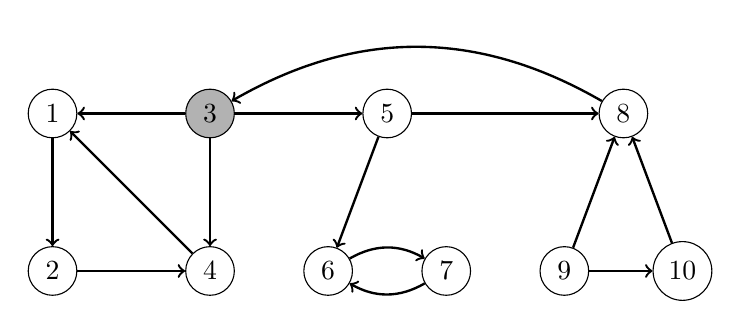
\begin{tikzpicture}[]
 \tikzset{gnode/.style ={fill=black!30!,circle,draw}}
 \tikzset{snode/.style ={fill=black!70!,circle,draw}}

 \node[circle,draw=black] (1) at (0,2) {$1$};
 \node[circle,draw=black] (2) at (0,0) {$2$};
 \node[gnode] (3) at (2,2) {$3$};
 \node[circle,draw=black] (4) at (2,0) {$4$};
 \node[circle,draw=black] (5) at (4.25,2) {$5$};
 \node[circle,draw=black] (6) at (3.5,0) {$6$};
 \node[circle,draw=black] (7) at (5,0) {$7$};
 \node[circle,draw=black] (8) at (7.25,2) {$8$};
 \node[circle,draw=black] (9) at (6.5,0) {$9$};
 \node[circle,draw=black] (10) at (8,0) {$10$};
		
 \draw[->,line width=0.3mm] (1) edge (2);
 \draw[->,line width=0.3mm] (2) edge (4);
 \draw[->,line width=0.3mm] (3) edge (1) (3) edge (4) (3) edge (5);
 \draw[->,line width=0.3mm] (4) edge (1);
 \draw[->,line width=0.3mm] (5) edge (6) (5) edge (8); 
 \draw[->,line width=0.3mm] (6) to[bend left] (7);
 \draw[->,line width=0.3mm] (7) to[bend left] (6);
 \draw[->,line width=0.3mm] (8) to[bend right] (3);
 \draw[->,line width=0.3mm] (9) edge (8) (9) edge (10);
 \draw[->,line width=0.3mm] (10) edge (8); 
\end{tikzpicture}
\hfill\,

\hfill
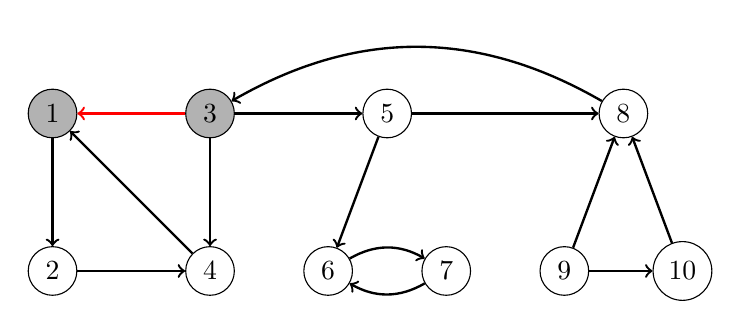
\begin{tikzpicture}[]
 \tikzset{gnode/.style ={fill=black!30!,circle,draw}}
 \tikzset{snode/.style ={fill=black!70!,circle,draw}}

 \node[gnode] (1) at (0,2) {$1$};
 \node[circle,draw=black] (2) at (0,0) {$2$};
 \node[gnode] (3) at (2,2) {$3$};
 \node[circle,draw=black] (4) at (2,0) {$4$};
 \node[circle,draw=black] (5) at (4.25,2) {$5$};
 \node[circle,draw=black] (6) at (3.5,0) {$6$};
 \node[circle,draw=black] (7) at (5,0) {$7$};
 \node[circle,draw=black] (8) at (7.25,2) {$8$};
 \node[circle,draw=black] (9) at (6.5,0) {$9$};
 \node[circle,draw=black] (10) at (8,0) {$10$};
		
 \draw[->,line width=0.3mm] (1) edge (2);
 \draw[->,line width=0.3mm] (2) edge (4);
 \draw[->,line width=0.3mm,red] (3) edge (1);
 \draw[->,line width=0.3mm] (3) edge (4) (3) edge (5);
 \draw[->,line width=0.3mm] (4) edge (1);
 \draw[->,line width=0.3mm] (5) edge (6) (5) edge (8); 
 \draw[->,line width=0.3mm] (6) to[bend left] (7);
 \draw[->,line width=0.3mm] (7) to[bend left] (6);
 \draw[->,line width=0.3mm] (8) to[bend right] (3);
 \draw[->,line width=0.3mm] (9) edge (8) (9) edge (10);
 \draw[->,line width=0.3mm] (10) edge (8); 
\end{tikzpicture}
\hfill\,

\hfill
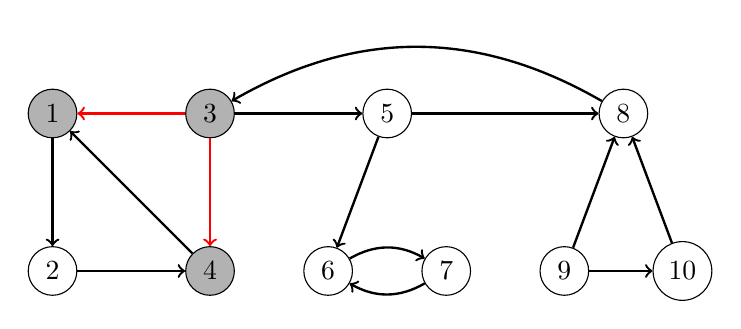
\begin{tikzpicture}[]
 \tikzset{gnode/.style ={fill=black!30!,circle,draw}}
 \tikzset{snode/.style ={fill=black!70!,circle,draw}}

 \node[gnode] (1) at (0,2) {$1$};
 \node[circle,draw=black] (2) at (0,0) {$2$};
 \node[gnode] (3) at (2,2) {$3$};
 \node[gnode] (4) at (2,0) {$4$};
 \node[circle,draw=black] (5) at (4.25,2) {$5$};
 \node[circle,draw=black] (6) at (3.5,0) {$6$};
 \node[circle,draw=black] (7) at (5,0) {$7$};
 \node[circle,draw=black] (8) at (7.25,2) {$8$};
 \node[circle,draw=black] (9) at (6.5,0) {$9$};
 \node[circle,draw=black] (10) at (8,0) {$10$};
		
 \draw[->,line width=0.3mm] (1) edge (2);
 \draw[->,line width=0.3mm] (2) edge (4);
 \draw[->,line width=0.3mm,red] (3) edge (1);
 \draw[->,line width=0.3mm,red] (3) edge (4);
 \draw[->,line width=0.3mm] (3) edge (5);
 \draw[->,line width=0.3mm] (4) edge (1);
 \draw[->,line width=0.3mm] (5) edge (6) (5) edge (8); 
 \draw[->,line width=0.3mm] (6) to[bend left] (7);
 \draw[->,line width=0.3mm] (7) to[bend left] (6);
 \draw[->,line width=0.3mm] (8) to[bend right] (3);
 \draw[->,line width=0.3mm] (9) edge (8) (9) edge (10);
 \draw[->,line width=0.3mm] (10) edge (8); 
\end{tikzpicture}
\hfill\,

\hfill
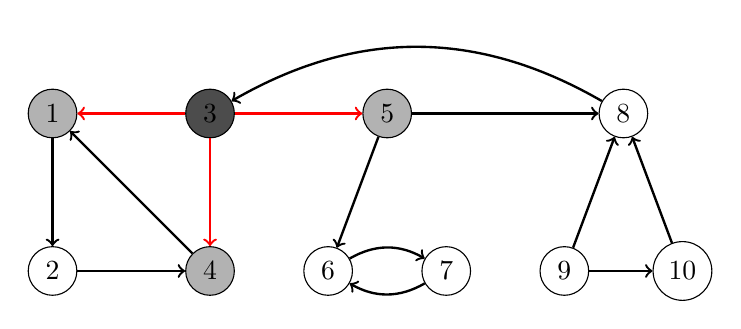
\begin{tikzpicture}[]
 \tikzset{gnode/.style ={fill=black!30!,circle,draw}}
 \tikzset{snode/.style ={fill=black!70!,circle,draw}}

 \node[gnode] (1) at (0,2) {$1$};
 \node[circle,draw=black] (2) at (0,0) {$2$};
 \node[snode] (3) at (2,2) {$3$};
 \node[gnode] (4) at (2,0) {$4$};
 \node[gnode] (5) at (4.25,2) {$5$};
 \node[circle,draw=black] (6) at (3.5,0) {$6$};
 \node[circle,draw=black] (7) at (5,0) {$7$};
 \node[circle,draw=black] (8) at (7.25,2) {$8$};
 \node[circle,draw=black] (9) at (6.5,0) {$9$};
 \node[circle,draw=black] (10) at (8,0) {$10$};
		
 \draw[->,line width=0.3mm] (1) edge (2);
 \draw[->,line width=0.3mm] (2) edge (4);
 \draw[->,line width=0.3mm,red] (3) edge (1);
 \draw[->,line width=0.3mm,red] (3) edge (4);
 \draw[->,line width=0.3mm,red] (3) edge (5);
 \draw[->,line width=0.3mm] (4) edge (1);
 \draw[->,line width=0.3mm] (5) edge (6) (5) edge (8); 
 \draw[->,line width=0.3mm] (6) to[bend left] (7);
 \draw[->,line width=0.3mm] (7) to[bend left] (6);
 \draw[->,line width=0.3mm] (8) to[bend right] (3);
 \draw[->,line width=0.3mm] (9) edge (8) (9) edge (10);
 \draw[->,line width=0.3mm] (10) edge (8); 
\end{tikzpicture}
\hfill\,

\hfill
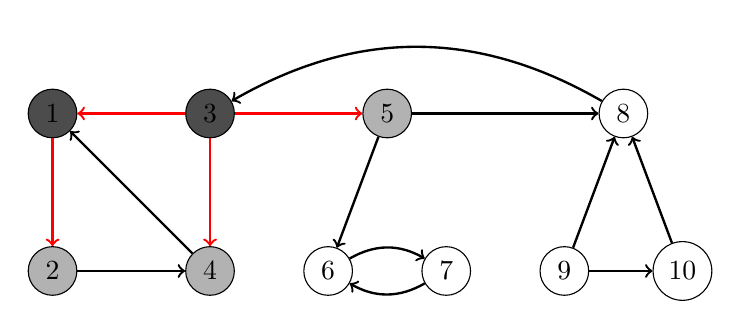
\begin{tikzpicture}[]
 \tikzset{gnode/.style ={fill=black!30!,circle,draw}}
 \tikzset{snode/.style ={fill=black!70!,circle,draw}}

 \node[snode] (1) at (0,2) {$1$};
 \node[gnode] (2) at (0,0) {$2$};
 \node[snode] (3) at (2,2) {$3$};
 \node[gnode] (4) at (2,0) {$4$};
 \node[gnode] (5) at (4.25,2) {$5$};
 \node[circle,draw=black] (6) at (3.5,0) {$6$};
 \node[circle,draw=black] (7) at (5,0) {$7$};
 \node[circle,draw=black] (8) at (7.25,2) {$8$};
 \node[circle,draw=black] (9) at (6.5,0) {$9$};
 \node[circle,draw=black] (10) at (8,0) {$10$};
		
 \draw[->,line width=0.3mm,red] (1) edge (2);
 \draw[->,line width=0.3mm] (2) edge (4);
 \draw[->,line width=0.3mm,red] (3) edge (1);
 \draw[->,line width=0.3mm,red] (3) edge (4);
 \draw[->,line width=0.3mm,red] (3) edge (5);
 \draw[->,line width=0.3mm] (4) edge (1);
 \draw[->,line width=0.3mm] (5) edge (6) (5) edge (8); 
 \draw[->,line width=0.3mm] (6) to[bend left] (7);
 \draw[->,line width=0.3mm] (7) to[bend left] (6);
 \draw[->,line width=0.3mm] (8) to[bend right] (3);
 \draw[->,line width=0.3mm] (9) edge (8) (9) edge (10);
 \draw[->,line width=0.3mm] (10) edge (8); 
\end{tikzpicture}
\hfill\,

\hfill
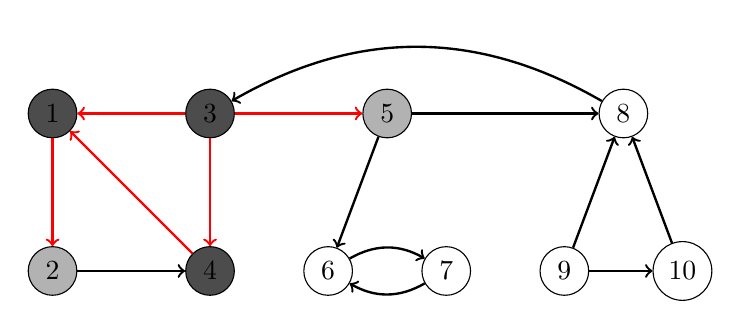
\begin{tikzpicture}[]
 \tikzset{gnode/.style ={fill=black!30!,circle,draw}}
 \tikzset{snode/.style ={fill=black!70!,circle,draw}}

 \node[snode] (1) at (0,2) {$1$};
 \node[gnode] (2) at (0,0) {$2$};
 \node[snode] (3) at (2,2) {$3$};
 \node[snode] (4) at (2,0) {$4$};
 \node[gnode] (5) at (4.25,2) {$5$};
 \node[circle,draw=black] (6) at (3.5,0) {$6$};
 \node[circle,draw=black] (7) at (5,0) {$7$};
 \node[circle,draw=black] (8) at (7.25,2) {$8$};
 \node[circle,draw=black] (9) at (6.5,0) {$9$};
 \node[circle,draw=black] (10) at (8,0) {$10$};
		
 \draw[->,line width=0.3mm,red] (1) edge (2);
 \draw[->,line width=0.3mm] (2) edge (4);
 \draw[->,line width=0.3mm,red] (3) edge (1);
 \draw[->,line width=0.3mm,red] (3) edge (4);
 \draw[->,line width=0.3mm,red] (3) edge (5);
 \draw[->,line width=0.3mm,red] (4) edge (1);
 \draw[->,line width=0.3mm] (5) edge (6) (5) edge (8); 
 \draw[->,line width=0.3mm] (6) to[bend left] (7);
 \draw[->,line width=0.3mm] (7) to[bend left] (6);
 \draw[->,line width=0.3mm] (8) to[bend right] (3);
 \draw[->,line width=0.3mm] (9) edge (8) (9) edge (10);
 \draw[->,line width=0.3mm] (10) edge (8); 
\end{tikzpicture}
\hfill\,

\hfill
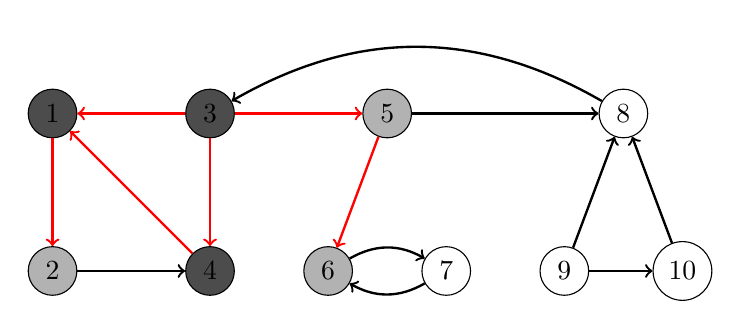
\begin{tikzpicture}[]
 \tikzset{gnode/.style ={fill=black!30!,circle,draw}}
 \tikzset{snode/.style ={fill=black!70!,circle,draw}}

 \node[snode] (1) at (0,2) {$1$};
 \node[gnode] (2) at (0,0) {$2$};
 \node[snode] (3) at (2,2) {$3$};
 \node[snode] (4) at (2,0) {$4$};
 \node[gnode] (5) at (4.25,2) {$5$};
 \node[gnode] (6) at (3.5,0) {$6$};
 \node[circle,draw=black] (7) at (5,0) {$7$};
 \node[circle,draw=black] (8) at (7.25,2) {$8$};
 \node[circle,draw=black] (9) at (6.5,0) {$9$};
 \node[circle,draw=black] (10) at (8,0) {$10$};
		
 \draw[->,line width=0.3mm,red] (1) edge (2);
 \draw[->,line width=0.3mm] (2) edge (4);
 \draw[->,line width=0.3mm,red] (3) edge (1);
 \draw[->,line width=0.3mm,red] (3) edge (4);
 \draw[->,line width=0.3mm,red] (3) edge (5);
 \draw[->,line width=0.3mm,red] (4) edge (1);
 \draw[->,line width=0.3mm,red] (5) edge (6);
 \draw[->,line width=0.3mm] (5) edge (8); 
 \draw[->,line width=0.3mm] (6) to[bend left] (7);
 \draw[->,line width=0.3mm] (7) to[bend left] (6);
 \draw[->,line width=0.3mm] (8) to[bend right] (3);
 \draw[->,line width=0.3mm] (9) edge (8) (9) edge (10);
 \draw[->,line width=0.3mm] (10) edge (8); 
\end{tikzpicture}
\hfill\,

\hfill
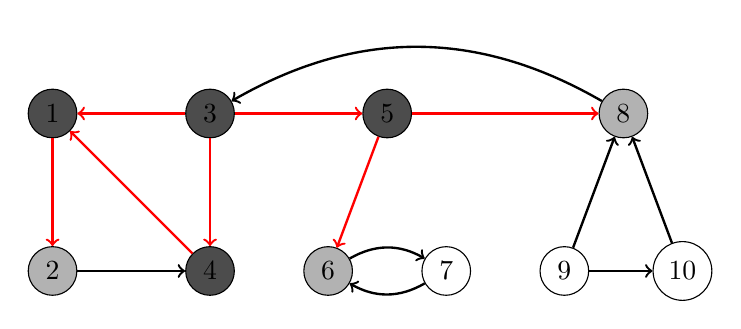
\begin{tikzpicture}[]
 \tikzset{gnode/.style ={fill=black!30!,circle,draw}}
 \tikzset{snode/.style ={fill=black!70!,circle,draw}}

 \node[snode] (1) at (0,2) {$1$};
 \node[gnode] (2) at (0,0) {$2$};
 \node[snode] (3) at (2,2) {$3$};
 \node[snode] (4) at (2,0) {$4$};
 \node[snode] (5) at (4.25,2) {$5$};
 \node[gnode] (6) at (3.5,0) {$6$};
 \node[circle,draw=black] (7) at (5,0) {$7$};
 \node[gnode] (8) at (7.25,2) {$8$};
 \node[circle,draw=black] (9) at (6.5,0) {$9$};
 \node[circle,draw=black] (10) at (8,0) {$10$};
		
 \draw[->,line width=0.3mm,red] (1) edge (2);
 \draw[->,line width=0.3mm] (2) edge (4);
 \draw[->,line width=0.3mm,red] (3) edge (1);
 \draw[->,line width=0.3mm,red] (3) edge (4);
 \draw[->,line width=0.3mm,red] (3) edge (5);
 \draw[->,line width=0.3mm,red] (4) edge (1);
 \draw[->,line width=0.3mm,red] (5) edge (6) (5) edge (8); 
 \draw[->,line width=0.3mm] (6) to[bend left] (7);
 \draw[->,line width=0.3mm] (7) to[bend left] (6);
 \draw[->,line width=0.3mm] (8) to[bend right] (3);
 \draw[->,line width=0.3mm] (9) edge (8) (9) edge (10);
 \draw[->,line width=0.3mm] (10) edge (8); 
\end{tikzpicture}
\hfill\,

Da die Knoten~$9$ und~$10$ nicht vom Startknoten $s=3$ aus erreichbar sind, ist der Endzustand nach dem Abschluss von $\cc{Breitensuche}(3)$ der folgende:

\hfill
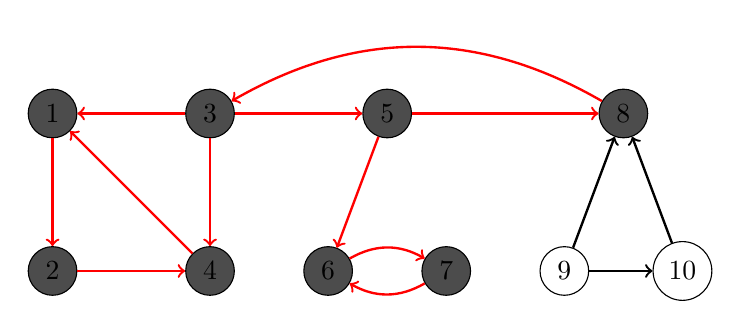
\begin{tikzpicture}[]
 \tikzset{gnode/.style ={fill=black!30!,circle,draw}}
 \tikzset{snode/.style ={fill=black!70!,circle,draw}}

 \node[snode] (1) at (0,2) {$1$};
 \node[snode] (2) at (0,0) {$2$};
 \node[snode] (3) at (2,2) {$3$};
 \node[snode] (4) at (2,0) {$4$};
 \node[snode] (5) at (4.25,2) {$5$};
 \node[snode] (6) at (3.5,0) {$6$};
 \node[snode] (7) at (5,0) {$7$};
 \node[snode] (8) at (7.25,2) {$8$};
 \node[circle,draw=black] (9) at (6.5,0) {$9$};
 \node[circle,draw=black] (10) at (8,0) {$10$};
		
 \draw[->,line width=0.3mm,red] (1) edge (2);
 \draw[->,line width=0.3mm,red] (2) edge (4);
 \draw[->,line width=0.3mm,red] (3) edge (1);
 \draw[->,line width=0.3mm,red] (3) edge (4) (3) edge (5);
 \draw[->,line width=0.3mm,red] (4) edge (1);
 \draw[->,line width=0.3mm,red] (5) edge (6) (5) edge (8); 
 \draw[->,line width=0.3mm,red] (6) to[bend left] (7);
 \draw[->,line width=0.3mm,red] (7) to[bend left] (6);
 \draw[->,line width=0.3mm,red] (8) to[bend right] (3);
 \draw[->,line width=0.3mm] (9) edge (8) (9) edge (10);
 \draw[->,line width=0.3mm] (10) edge (8); 
\end{tikzpicture}
\hfill\,
\end{beispiel}

Der Beweis der Korrektheit der Breitensuche inklusive der korrekten Bestimmung der Abstände $\delta(s,v)$, für $v \in V$, erfordert noch etwas Vorbereitung.
Die Laufzeitanalyse können wir allerdings bereits durchführen, mit dem Ergebnis, dass auch die Breitensuche einen optimalen linearen Aufwand erfordert:

\begin{theorem}
\label{thm:laufzeit-breitensuche}
Es sei ein Digraph $D=(V,A)$ durch eine Adjazenzliste gegeben und es sei $s \in V$ ein beliebiger Startknoten.
Die Laufzeit von $\cc{Breitensuche}(s)$ ist $\Theta(|V|+|A|)$.
\end{theorem}

\begin{proof}
Der Aufwand für die Initialisierung $\cc{Breitensuche-initialisieren}(D,s)$ ist direkt als $\Theta(|V|)$ festzustellen.

Nach der Initialisierung wird nie mehr ein Knoten weiß gefärbt und der Test in Zeile~\ref{line:breitensuche-if} von $\cc{Breitensuche}(s)$ stellt sicher, dass jeder Knoten~$v$ nur ein Mal in die Warteschlange eingefügt und aus ihr entnommen wird.
Da die Operationen $\cc{Dequeue}(Q)$ und $\cc{Enqueue}(Q,v)$ konstanten Aufwand haben, benötigen wir für alle Warteschlangenoperationen zusammen $\Theta(|V|)$ Zeiteinheiten.

Desweiteren wird die Nachbarschaft $N[u]$ eines Knotens~$u$ nur dann durchsucht, wenn~$u$ aus der Warteschlange entnommen wird.
Die Adjazenzliste wird daher nur ein Mal durchsucht, was einen zusätzlichen Aufwand von $\Theta(|A|)$ ergibt. 

Zusammenfassend erhalten wir also  wie behauptet einen Zeitaufwand von $\Theta(|V|) + \Theta(|V|) + \Theta(|A|) = \Theta(|V|+|A|)$.
\end{proof}


\subsubsection{Eigenschaften der Breitensuche}
\label{sect:breitensuche-eigenschaften}

Nachfolgend studieren wir wichtige Eigenschaften der Breitensuche, mit deren Hilfe wir beweisen werden, dass die Breitensuche die Distanzen $\delta(s,v)$ vom Startknoten~$s$ zu allen anderen Knoten des gegebenen Digraphen $D=(V,A)$ korrekt bestimmt.
Wir nennen einen $(s,v)$-Pfad der Länge $\delta(s,v)$ einen \emph{kürzesten Pfad} von~$s$ nach~$v$ in~$D$.

\begin{lemma}
\label{lem:breitensuche-pfad-dreieck}
Sei $D=(V,A)$ ein Digraph und sei $s \in V$ ein beliebiger Startknoten.
Dann gilt für jede Kante $(u,v) \in A$, dass
\[
\delta(s,v) \leq \delta(s,u) + 1.
\]
\end{lemma}

\begin{proof}
Falls $u$ von $s$ aus erreichbar ist, dann ist es auch~$v$.
In diesem Fall ist der kürzeste $(s,v)$-Pfad nicht länger als der kürzeste $(s,u)$-Pfad, verlängert um die Kante $(u,v)$, und die Ungleichung gilt.
Ist~$u$ nicht von~$s$ aus erreichbar, so ist $\delta(s,u)=\infty$, und die Ungleichung ist trivialerweise erfüllt.
\end{proof}

Auf der Grundlage dieser einfachen Eigenschaft lässt sich zunächst einmal zeigen, dass das Attribut $d[v]$ stets eine obere Schranke an die Länge eines kürzesten $(s,v)$-Pfades liefert.

\begin{lemma}
\label{lem:breitensuche-d-geq-delta}
Sei $D=(V,A)$ ein Digraph und sei $s \in V$ ein beliebiger Knoten.
Nach Abschluss der Prozedur $\cc{Breitensuche}(s)$ gilt $d[v] \geq \delta(s,v)$, für alle $v \in V$.
\end{lemma}

\begin{proof}
Wir argumentieren mittels vollständiger Induktion nach der Anzahl der Einfügeoperationen in die Warteschlange~$Q$.

Der Induktionsanfang ist der Zeitpunkt nach der Initialisierung zu dem $d[s]=0=\delta(s,s)$ und, für alle $v \in V \setminus \{s\}$, die Ungleichung $d[v]=\infty\geq\delta(s,v)$ gilt.

Für den Induktionsschritt sei~$v$ ein weißer Knoten, der bei der Suche vom Knoten~$u$ aus entdeckt wird.
Nach Induktionsvoraussetzung gilt $d[u] \geq \delta(s,u)$.
Aufgrund der Zuweisung in Zeile~\ref{line:breitensuche-d} in $\cc{Breitensuche}(s)$ und Lemma~\ref{lem:breitensuche-pfad-dreieck} gilt
\[
d[v] = d[u] + 1 \geq \delta(s,u) + 1 \geq \delta(s,v).
\]
Der Knoten~$v$ wird in die Warteschlange~$Q$ eingefügt, und da er zu diesem Zeitpunkt grau gefärbt wurde, ändert sich der Wert $d[v]$ nicht mehr und die Ungleichung bleibt bis zur Terminierung des Algorithmus gültig.
\end{proof}

Bevor wir die umgekehrte Ungleichung beweisen können, müssen wir die Arbeitsweise der Warteschlange~$Q$ besser verstehen.
Es zeigt sich, dass~$Q$ zu jedem Zeitpunkt nur höchstens zwei verschiedene Werte von~$d$ enthält.
Wir fassen dafür die Warteschlange als Liste oder Array $[v_1,\ldots,v_r]$ auf, wobei $v_1$ der Kopf und $v_r$ das Ende von~$Q$ ist.

\begin{lemma}
\label{lem:breitensuche-warteschlange-monotonie}
Zu jedem Zeitpunkt der Ausführung von $\cc{Breitensuche}(s)$ erfüllt die Warteschlange $Q=[v_1,\ldots,v_r]$ die Bedingung
\[
d[v_1] \leq d[v_2] \leq \ldots \leq d[v_r] \leq d[v_1] + 1.
\]
\end{lemma}

\begin{proof}
Ganz am Anfang der Breitensuche enthält~$Q$ nur den Startknoten~$s$ und die Aussage gilt trivialerweise.

Wir zeigen nun, dass wenn die behauptete Bedingung zu einem Zeitpunkt gilt, dass sie auch dann gültig bleibt, wenn eine Warteschlangenoperation ausgeführt wird.
(Das heißt, wir argumentieren mittels vollständiger Induktion über die Anzahl der ausgeführten Warteschlangenoperationen.)

Sei zunächst wie angenommen $Q=[v_1,\ldots,v_r]$ und führen wir $\cc{Dequeue}(Q)$ aus.
Das heißt, $v_1$ wird aus $Q$ entfernt und $v_2$ wird der neue Kopf der Warteschlange.
Da nach Annahme $d[v_1] \leq d[v_2]$ gilt, haben wir $d[v_r] \leq d[v_1]+1 \leq d[v_2]+1$.
Da außerdem alle anderen Ungleichungen unverändert bleiben, gilt die behauptete Kette von Ungleichungen für die neue Warteschlange $Q'=[v_2,\ldots,v_r]$.

Schauen wir uns nun an was passiert wenn in Zeile~\ref{line:breitensuche-enqueue} von $\cc{Breitensuche}(s)$ die Operation $\cc{Enqueue}(Q,v)$ ausgeführt wird.
Der Knoten~$v$ wird zum Ende der neuen Warteschlange $Q'=[v_1,\ldots,v_r,v]$ und zum Zeitpunkt dieser Operation durchsucht der Algorithmus die Nachbarschaft des Knotens~$u$, der zuvor aus der Warteschlange entfernt wurde.
Daher gilt nach Annahme die Ungleichung $d[u] \leq d[v_i]$ für alle $1 \leq i \leq r$ und nach Zeile~\ref{line:breitensuche-d} weiterhin $d[v] = d[u]+1 \leq d[v_1]+1$.
Es gilt außerdem, dass $d[v_r] \leq d[u]+1=d[v]$, da wie bereits erwähnt, $u$ zuvor aus der Schlange entfernt wurde, und nach Annahme die Aussage des Lemmas vor der Operation $\cc{Enqueue}(Q,v)$ gilt.
Alle anderen Ungleichungen bleiben unangetastet und wir erhalten zusammenfassend
\[
d[v_1] \leq d[v_2] \leq \ldots d[v_r] \leq d[v] \leq d[v_1] + 1,
\]
wie gewünscht.
\end{proof}

\begin{corollary}
\label{cor:breitensuche-warteschlange}
Nehmen wir an die Knoten~$v_i$ und $v_j$ würden während der Ausführung von $\cc{Breitensuche}(s)$ in die Warteschlange~$Q$ eingefügt, und nehmen wir weiterhin an, dass~$v_i$ vor $v_j$ eingefügt wird.
Dann gilt $d[v_i] \leq d[v_j]$ zum Zeitpunkt des Einfügens von~$v_j$.
\end{corollary}

\begin{proof}
Die Aussage folgt direkt aus Lemma~\ref{lem:breitensuche-warteschlange-monotonie} und der Beobachtung, dass jeder Knoten während der Ausführung von $\cc{Breitensuche}(s)$ höchstens einmal einen endlichen Wert für~$d$ zugewiesen bekommt.
\end{proof}

Wir sind nun in der Lage die Korrektheit des Algorithmus zur Breitensuche zu beweisen und die Bestimmung der Abstände $\delta(s,v)$, für $v \in V$, zu vervollständigen.

\begin{theorem}
\label{thm:breitensuche}
Sei $D=(V,A)$ ein Digraph und sei $s \in V$ ein beliebiger Knoten.
Dann entdeckt die Prozedur $\cc{Breitensuche}(s)$ während ihrer Ausführung jeden Knoten, der von~$s$ aus erreichbar ist, und bei der Terminierung gilt $d[v] = \delta(s,v)$, für alle $v \in V$.

Außerdem besteht für jeden von~$s$ aus erreichbaren Knoten $v \neq s$, einer der kürzesten $(s,v)$-Pfade aus einem kürzesten $(s,\pi[v])$-Pfad und der Kante $(\pi[v],v)$.
\end{theorem}

\begin{proof}
Wir führen einen Widerspruchsbeweis und nehmen dazu an, dass es einen Knoten~$v$ gibt, so dass $d[v] \neq \delta(s,v)$ gilt.
Sei weiterhin angenommen, dass~$v$ ein solcher Knoten mit kleinstem Abstand $\delta(s,v)$ zu~$s$ ist.
Da $d[s]=0=\delta(s,s)$ gilt, ist demnach in jedem Fall $v \neq s$.
Nach Lemma~\ref{lem:breitensuche-d-geq-delta} ist $d[v] \geq \delta(s,v)$ und daher $d[v] > \delta(s,v)$ für diesen ausgezeichneten Knoten~$v$.
Weiterhin muss~$v$ von~$s$ aus erreichbar sein, da ansonsten $\delta(s,v)=\infty \geq d[v]$ gelte.
Sei nun~$u$ ein Knoten auf einem kürzesten $(s,v)$-Pfad, der unmittelbar vor~$v$ liegt, so dass $\delta(s,v)=\delta(s,u)+1$ gilt.
Die Wahl des Knotens~$v$ zusammen mit $\delta(s,u) < \delta(s,v)$ ergibt die Identität $d[u]=\delta(s,u)$, und wir fassen unsere Beobachtungen in folgender Ungleichungskette zusammen
\begin{align}
d[v] &> \delta(s,v) = \delta(s,u) + 1 = d[u] + 1.\label{eqn:breitensuche-korrekt}
\end{align}

Sehen wir uns den Zeitpunkt an, zu dem der Algorithmus $\cc{Breitensuche}(s)$ in Zeile~\ref{line:breitensuche-dequeue} den Knoten~$u$ aus der Warteschlange entfernt.
Wir unterscheiden danach, welche Farbe $\cc{Farbe}[v]$ der Knoten~$v$ zu diesem Zeitpunkt trägt:

Ist $\cc{Farbe}[v]=\cc{weiss}$, so wird in Zeile~\ref{line:breitensuche-d} $d[v]=d[u]+1$ gesetzt und danach im Algorithmus nicht mehr verändert.
Dies steht im Widerspruch zu~\eqref{eqn:breitensuche-korrekt}.

Ist $\cc{Farbe}[v]=\cc{grau}$, so ist er beim Entfernen eines anderen Knotens~$w$ aus der Warteschlange grau gefärbt worden.
Dieser Knoten wurde früher als~$u$ aus der Warteschlange entfernt und es wurde $d[v]=d[w]+1$ gesetzt.
Nach Korollar~\ref{cor:breitensuche-warteschlange} gilt daher $d[w] \leq d[u]$ und damit $d[v]=d[w]+1 \leq d[u]+1$, im Widerspruch zu~\eqref{eqn:breitensuche-korrekt}.

Ist $\cc{Farbe}[v]=\cc{schwarz}$, so wurde~$v$ bereits aus der Warteschlange entfernt und nach Korollar~\ref{cor:breitensuche-warteschlange} gilt $d[v] \leq d[u]$, im Widerspruch zu~\eqref{eqn:breitensuche-korrekt}.

Zusammenfassend erhalten wir in jedem Fall einen Widerspruch zu~\eqref{eqn:breitensuche-korrekt} und damit gilt also $d[v]=\delta(s,v)$, für alle Knoten $v \in V$.
Alle von~$s$ aus erreichbaren Knoten werden bei der Breitensuche entdeckt, da für einen ansonsten unentdeckten Knoten~$v$ der Initialwert $d[v]=\infty$ größer als $\delta(s,v)$ wäre.
Abschließend bemerken wir noch, dass die Verwaltung der Vorgängerabbildung~$\pi$ und des Abstandsattributs~$d$ in den Zeilen~\ref{line:breitensuche-pi} und~\ref{line:breitensuche-d} von $\cc{Breitensuche}(s)$ impliziert, dass $\delta(s,v)=d[v]=d[\pi[v]]+1=\delta(s,\pi[v])+1$ gilt und somit jeder kürzeste $(s,\pi[v])$-Pfad über die Kante $(\pi[v],v)$ zu einem kürzesten $(s,v)$-Pfad erweitert werden kann.
\end{proof}


Analog zur Tiefensuche erzeugt die Vorgängerabbildung $\pi$ auch bei der Breitensuche auf einem Digraphen $D=(V,A)$, die von einem Startknoten~$s \in V$ ausgeht, einen \emph{Vorgängerteilgraphen} $D_\pi = (V_\pi,A_\pi)$, der durch
\[
V_\pi := \left\{ v \in V : \pi[v] \neq \cc{nil}\right\} \cup \{s\} \quad \text{ und } \quad A_\pi := \left\{ (\pi[v],v) : v \in V_\pi \setminus \{s\}\right\}
\]
definiert ist.

Da $D_\pi$ nach Definition zusammenhängend ist und da die Gleichung $|A_\pi|=|V_\pi|-1$ besteht, ist der Vorgängerteilgraph stets ein Baum.
Daher nennen wir die Kanten in $A_\pi \subseteq A$ wieder \emph{Baumkanten} der Breitensuche und den Graphen~$D_\pi$ den zugehörigen \emph{Breitensuchbaum}.

\begin{beispiel}
Sammeln wir die Daten zur Vorgängerabbildung und zu den Distanzen während der Breitensuche in Beispiel~\ref{bsp:breitensuche}, so erhalten wir nach Abschluss von $\cc{Breitensuche}(3)$ die folgenden Werte:

\begin{table}[H]
\centering
\begin{tabular}{|c|c|c|c|c|c|c|c|c|c|c|}
\hline
\textbf{Knoten $u$}        & \textbf{1} & \textbf{2} & \textbf{3} & \textbf{4} & \textbf{5} & \textbf{6} & \textbf{7} & \textbf{8} & \textbf{9} & \textbf{10} \\ \hline
\textbf{$\pi[u]$}    & 3          & 1          & $\cc{nil}$          & 3          & 3          & 5          & 6         & 5         & $\cc{nil}$         & $\cc{nil}$          \\ \hline
\textbf{$d[u]$} & 1          & 2          & 0         & 1          & 1         & 2         & 3         & 2         & $\infty$         & $\infty$          \\ \hline
\end{tabular}
\end{table}

Daraus ergibt sich der nachfolgende Breitensuchbaum, in dem der kürzeste $(3,7)$-Pfad in blau markiert ist:

\hfill
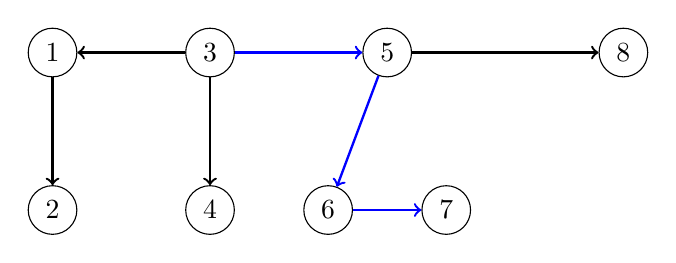
\begin{tikzpicture}[]
 \node[circle,draw=black] (1) at (0,2) {$1$};
 \node[circle,draw=black] (2) at (0,0) {$2$};
 \node[circle,draw=black] (3) at (2,2) {$3$};
 \node[circle,draw=black] (4) at (2,0) {$4$};
 \node[circle,draw=black] (5) at (4.25,2) {$5$};
 \node[circle,draw=black] (6) at (3.5,0) {$6$};
 \node[circle,draw=black] (7) at (5,0) {$7$};
 \node[circle,draw=black] (8) at (7.25,2) {$8$};
% \node[circle,draw=black] (9) at (6.5,0) {$9$};
% \node[circle,draw=black] (10) at (8,0) {$10$};
		
 \draw[->,line width=0.3mm] (1) edge (2);
 \draw[->,line width=0.3mm] (3) edge (4);
 \draw[->,line width=0.3mm] (3) edge (1) ;
 \draw[->,line width=0.3mm] (5) edge (8); 
 \draw[->,line width=0.3mm,blue] (3) edge (5) (5) edge (6) (6) edge (7);
\end{tikzpicture}
\hfill\,

Beachten Sie, dass die Knoten $9$ und $10$ nicht im Breitensuchbaum auftreten, da diese vom Startknoten~$s=3$ aus nicht erreichbar sind.
\end{beispiel}

Eine weitere wichtige Eigenschaft des Breitensuchbaumes ist, dass er kürzeste Pfade von~$s$ zu allen erreichbaren Knoten enthält:

\begin{aufgabe}
Der Breitensuchbaum~$D_\pi$ besteht aus genau den Knoten in~$V$, die von $s$ aus erreichbar sind, und für jeden Knoten $v \in V_\pi$ enthält~$D_\pi$ einen einzigen Weg von~$s$ nach~$v$, der zugleich ein kürzester $(s,v)$-Pfad in~$D$ ist.
\end{aufgabe}

Um einen solchen kürzesten $(s,v)$-Pfad zu bestimmen kann man die Vorgänger-Abbildung~$\pi$ rekursiv benutzen um \glqq sich von~$v$ zurück zu~$s$ zu hangeln\grqq.
Die folgende Prozedur gibt die Knoten entlang eines solchen Pfades aus, wenn er denn existiert:

\begin{algorithm}[H]
\caption{$\cc{Pfad-Ausgeben}(D,s,v)$}
\begin{algorithmic}[1]
 \IF{$v=s$}
  \STATE print $s$
 \ELSIF{$\pi[v]=\cc{nil}$}
  \STATE print \glqq Es gibt keinen Pfad von $s$ nach $v$.\grqq
 \ELSE
  \STATE $\cc{Pfad-Ausgeben}(D,s,\pi[v])$
  \STATE print $v$
 \ENDIF
\end{algorithmic}
\end{algorithm}

Die Laufzeit dieser Prozedur ist proportional zu der Anzahl der Knoten auf dem ausgegebenen $(s,v)$-Pfad, da jeder rekursive Aufruf für einen Pfad erfolgt, der einen Knoten kürzer ist.
Das heißt, die Laufzeit ist~$\Theta(\delta(s,v)) \subseteq O(|V|)$, falls~$v$ von~$s$ aus erreichbar ist, und $\Theta(1)$ sonst.


\begin{remark}
Analog zur diskutierten Breitensuche kann man eine \emph{Tiefensuche} auch ohne Rekursion umsetzen.
(Dies hat gewisse Vorteile, weil der Programmstack nicht zu sehr belastet wird.)
Dazu ersetzt man die Warteschlange $Q$ durch einen sogennanten \emph{Stack} (oder \emph{Stapel}). 

Ein Stack ist eine Liste $S=[s_1,\ldots,s_k]$ mit ebenfalls zwei Grundoperationen:
\begin{itemize}
 \item $\cc{Pop}(S)$: Das \emph{letzte} Element~$s_k$ von~$S$ wird zurückgegeben und entfernt.

 \item $\cc{Push}(S,x)$: Das Element~$x$ wird am \emph{Ende} von~$S$ hinzugefügt.
\end{itemize}

Ein Stack arbeitet also nach dem LIFO-Prinzip (Last In - First Out).
\end{remark}